% questions.tex —— 2009 年·普通高等学校招生考试·天津卷·理科 · 题目内容片段（无答案）
% 由 tools/generate_projects.py 依来源总账自 2009/2009_数学真题_天津理_试题.md 生成，勿手改（改源 MD 后重跑）


状态：needs-review；依固定候选 PDF 两页（印刷页 561–562）逐题核验，图形已矢量重绘，正式构建与逐页验收见回执。源未标分值，不补分值。

\gkpart{一、选择题}

\begin{question}
\gkti{1}$\mathrm i$ 是虚数单位，$\dfrac{5\mathrm i}{2-\mathrm i}=$（　）

（A）$1+2\mathrm i$

（B）$-1-2\mathrm i$

（C）$1-2\mathrm i$

（D）$-1+2\mathrm i$

\end{question}
\begin{question}
\gkti{2}设变量 $x,y$ 满足约束条件 $\begin{cases}x+y\geqslant3,\\ x-y\geqslant-1,\\ 2x-y\leqslant3,\end{cases}$ 则目标函数 $z=2x+3y$ 的最小值为（　）

（A）$6$

（B）$7$

（C）$8$

（D）$23$

\end{question}
\begin{question}
\gkti{3}命题「存在 $x_0\in\mathbf R$，$2^{x_0}\leqslant0$」的否定是（　）

（A）不存在 $x_0\in\mathbf R$，$2^{x_0}>0$

（B）存在 $x_0\in\mathbf R$，$2^{x_0}\geqslant0$

（C）对任意的 $x\in\mathbf R$，$2^x\leqslant0$

（D）对任意的 $x\in\mathbf R$，$2^x>0$

\end{question}
\begin{question}
\gkti{4}设函数 $f(x)=\dfrac13x-\ln x$（$x>0$），则 $y=f(x)$（　）

（A）在区间 $\left(\dfrac1e,1\right)$，$(1,\mathrm e)$ 内均有零点

（B）在区间 $\left(\dfrac1e,1\right)$，$(1,\mathrm e)$ 内均无零点

（C）在区间 $\left(\dfrac1e,1\right)$ 内有零点，在区间 $(1,\mathrm e)$ 内无零点

（D）在区间 $\left(\dfrac1e,1\right)$ 内无零点，在区间 $(1,\mathrm e)$ 内有零点

\Needspace{0.4\textheight}
\end{question}
\begin{question}
\gkti{5}阅读如图的程序框图，则输出的 $S=$（　）
\nopagebreak[4]
\begin{center}% 2009 年天津卷理科第 5 题：求 S=2+5+8+11+14 的程序框图。
% 来源 PDF：普通高考/2009/2009天津理.pdf，SHA256 ea758271e47ecf0aadf9b6ea943bcdf2df78b8bf284c3ef26b72c4b69eeb3e80
% 原页：第 1 页（A3 三栏）第 1 栏下部，印刷页 561。
% 重绘依据：开始 → S=0,i=1 → T=3i-1 → S=S+T → i=i+1 → 判断 i>5；否（右）回到 T=3i-1，
%   是（下）→ 输出 S → 结束。
\begin{tikzpicture}[scale=0.9, semithick, >=Stealth,
  node distance=5mm, every node/.style={inner sep=3pt, font=\small}]
  \node (start) [draw, rounded corners=4pt, minimum width=2.0cm, minimum height=0.65cm] {开始};
  \node (init) [draw, minimum width=3.2cm, minimum height=0.65cm, below=of start] {$S=0,\ i=1$};
  \node (t) [draw, minimum width=3.2cm, minimum height=0.65cm, below=of init] {$T=3i-1$};
  \node (add) [draw, minimum width=3.2cm, minimum height=0.65cm, below=of t] {$S=S+T$};
  \node (inc) [draw, minimum width=3.2cm, minimum height=0.65cm, below=of add] {$i=i+1$};
  \node (cond) [draw, diamond, aspect=2.0, minimum width=3.0cm, minimum height=1.0cm, below=of inc] {$i>5$};
  \node (out) [draw, trapezium, trapezium left angle=70, trapezium right angle=110,
    minimum width=2.8cm, minimum height=0.65cm, below=of cond] {输出 $S$};
  \node (end) [draw, rounded corners=4pt, minimum width=2.0cm, minimum height=0.65cm, below=of out] {结束};
  \draw[->] (start) -- (init);
  \draw[->] (init) -- (t);
  \draw[->] (t) -- (add);
  \draw[->] (add) -- (inc);
  \draw[->] (inc) -- (cond);
  \draw[->] (cond) -- (out);
  \node[anchor=west] at ($(cond.south)!0.5!(out.north)+(20pt,-6pt)$) {是};
  \draw[->] (cond.east) -- ++(1.1,0) |- node[pos=0.25, right] {否} (t.east);
  \draw[->] (out) -- (end);
\end{tikzpicture}
\end{center}
\nopagebreak[4]
（A）$26$

（B）$35$

（C）$40$

（D）$57$

\end{question}
\begin{question}
\gkti{6}设 $a>0$，$b>0$．若 $\sqrt3$ 是 $3^a$ 与 $3^b$ 的等比中项，则 $\dfrac1a+\dfrac1b$ 的最小值为（　）

（A）$8$

（B）$4$

（C）$1$

（D）$\dfrac14$

\end{question}
\begin{question}
\gkti{7}已知函数 $f(x)=\sin\left(\omega x+\dfrac{\pi}{4}\right)$（$x\in\mathbf R$，$\omega>0$）的最小正周期为 $\pi$．为了得到函数 $g(x)=\cos\omega x$ 的图象，只要将 $y=f(x)$ 的图象（　）

（A）向左平移 $\dfrac{\pi}{8}$ 个单位长度

（B）向右平移 $\dfrac{\pi}{8}$ 个单位长度

（C）向左平移 $\dfrac{\pi}{4}$ 个单位长度

（D）向右平移 $\dfrac{\pi}{4}$ 个单位长度

\end{question}
\begin{question}
\gkti{8}已知函数 $f(x)=\begin{cases}x^2+4x,&x\geqslant0,\\ 4x-x^2,&x<0.\end{cases}$ 若 $f(2-a^2)>f(a)$，则实数 $a$ 的取值范围是（　）

（A）$(-\infty,-1)\cup(2,+\infty)$

（B）$(-1,2)$

（C）$(-2,1)$

（D）$(-\infty,-2)\cup(1,+\infty)$

\end{question}
\begin{question}
\gkti{9}设抛物线 $y^2=2x$ 的焦点为 $F$，过点 $M(\sqrt3,0)$ 的直线与抛物线相交于 $A,B$ 两点，与抛物线的准线相交于 $C$，$|BF|=2$，则 $\triangle BCF$ 与 $\triangle ACF$ 的面积之比 $\dfrac{S_{\triangle BCF}}{S_{\triangle ACF}}=$（　）

（A）$\dfrac45$

（B）$\dfrac23$

（C）$\dfrac47$

（D）$\dfrac12$

\end{question}
\begin{question}
\gkti{10}$0<b<1+a$．若关于 $x$ 的不等式 $(x-b)^2>(ax)^2$ 的解集中的整数恰有 $3$ 个，则（　）

（A）$-1<a<0$

（B）$0<a<1$

（C）$1<a<3$

（D）$3<a<6$

\end{question}
\gkpart{二、填空题}

\begin{question}
\gkti{11}某学院的 $A,B,C$ 三个专业共有 $1200$ 名学生，为了调查这些学生勤工俭学的情况，拟采用分层抽样的方法抽取一个容量为 $120$ 的样本．已知该学院的 $A$ 专业有 $380$ 名学生，$B$ 专业有 $420$ 名学生，则在该学院的 $C$ 专业应抽取\gkblank{}名学生．

\Needspace{0.4\textheight}
\end{question}
\begin{question}
\gkti{12}如图是一个几何体的三视图，若它的体积是 $3\sqrt3$，则 $a=$\gkblank{}．
\nopagebreak[4]
\begin{center}% 2009 年天津卷理科第 12 题：直三棱柱的三视图。
% 来源 PDF：普通高考/2009/2009天津理.pdf，SHA256 ea758271e47ecf0aadf9b6ea943bcdf2df78b8bf284c3ef26b72c4b69eeb3e80
% 原页：第 1 页（A3 三栏）第 2 栏中部，印刷页 561。
% 重绘依据：正视图为 3×a 矩形；侧视图为底边 2、高 a 的三角形；俯视图为 3×2 矩形，
%   中间一条平行于长的实线把深度分成 1 与 1 两段；尺寸与标注按原图。
\begin{tikzpicture}[scale=0.95, semithick, every node/.style={inner sep=1.2pt}]
  % 正视图
  \draw (0,1.5) rectangle (3,3.0);
  \node[anchor=east] at (-0.1,2.25) {$a$};
  \node[anchor=north] at (1.5,1.35) {正视图};
  % 侧视图
  \draw (4.2,1.5) -- (5.8,1.5) -- (5.0,3.0) -- cycle;
  \node[anchor=north] at (5.0,1.05) {侧视图};
  \node[anchor=north] at (5.0,1.32) {$2$};
  % 俯视图
  \draw (0,-0.35) rectangle (3,0.65);
  \draw (0,0.15) -- (3,0.15);
  \node[anchor=north] at (1.5,-0.5) {俯视图};
  \node[anchor=east] at (-0.1,-0.1) {$1$};
  \node[anchor=east] at (-0.1,0.4) {$1$};
\end{tikzpicture}
\end{center}
\nopagebreak[4]
\end{question}
\begin{question}
\gkti{13}设直线 $l_1$ 的参数方程为 $\begin{cases}x=1+t,\\ y=1+3t,\end{cases}$（$t$ 为参数），直线 $l_2$ 的方程为 $y=3x+4$，则 $l_1$ 与 $l_2$ 的距离为\gkblank{}．

\end{question}
\begin{question}
\gkti{14}若圆 $x^2+y^2=4$ 与圆 $x^2+y^2+2ay-6=0$（$a>0$）的公共弦的长为 $2\sqrt3$，则 $a=$\gkblank{}．

\end{question}
\begin{question}
\gkti{15}在四边形 $ABCD$ 中，$\overrightarrow{AB}=\overrightarrow{DC}=(1,1)$，$\dfrac{1}{|\overrightarrow{BA}|}\overrightarrow{BA}+\dfrac{1}{|\overrightarrow{BC}|}\overrightarrow{BC}=\dfrac{\sqrt3}{|\overrightarrow{BD}|}\overrightarrow{BD}$，则四边形 $ABCD$ 的面积为\gkblank{}．

\end{question}
\begin{question}
\gkti{16}用数字 $0,1,2,3,4,5,6$ 组成没有重复数字的四位数，其中个位、十位和百位上的数字之和为偶数的四位数共有\gkblank{}个．（用数字作答）

\end{question}
\gkpart{三、解答题}

\begin{question}
\gkti{17}在 $\triangle ABC$ 中，$BC=\sqrt5$，$AC=3$，$\sin C=2\sin A$．

（1）求 $AB$ 的值；

（2）求 $\sin\left(2A-\dfrac{\pi}{4}\right)$ 的值．

\end{question}
\begin{question}
\gkti{18}在 $10$ 件产品中，有 $3$ 件一等品，$4$ 件二等品，$3$ 件三等品．从这 $10$ 件产品中任取 $3$ 件，求：

（1）取出的 $3$ 件产品中一等品件数 $X$ 的分布列和数学期望；

（2）取出的 $3$ 件产品中一等品件数多于二等品件数的概率．

\Needspace{0.4\textheight}
\end{question}
\begin{question}
\gkti{19}如图，在五面体 $ABCDEF$ 中，$FA\perp$ 平面 $ABCD$，$AD\parallel BC\parallel FE$，$AB\perp AD$，$M$ 为 $EC$ 的中点，$AF=AB=BC=FE=\dfrac12AD$．
\nopagebreak[4]
\begin{center}% 2009 年天津卷理科第 19 题：五面体 ABCDEF，FA⊥平面 ABCD，AD∥BC∥FE。
% 来源 PDF：普通高考/2009/2009天津理.pdf，SHA256 ea758271e47ecf0aadf9b6ea943bcdf2df78b8bf284c3ef26b72c4b69eeb3e80
% 原页：第 2 页（A3 三栏）第 1 栏上部，印刷页 562。
% 重绘依据：A 前左下、B 前右下、C 右后、D 左后；F 在 A 正上方，E 在 F 后上方且 FE∥AD；
%   M 为 EC 中点。被遮挡的 D-A 画虚线。
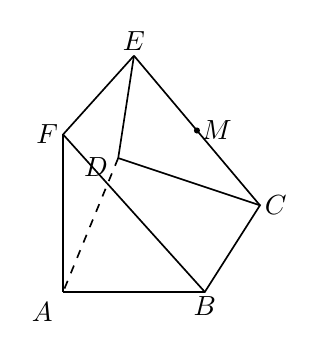
\begin{tikzpicture}[scale=1.0, semithick, every node/.style={inner sep=1.5pt}]
  \coordinate (A) at (0,0);
  \coordinate (B) at (1.8,0);
  \coordinate (C) at (2.5,1.1);
  \coordinate (D) at (0.7,1.7);
  \coordinate (F) at (0,2.0);
  \coordinate (E) at (0.9,3.0);
  \coordinate (M) at (1.7,2.05);
  % 底面
  \draw (A) -- (B) -- (C) -- (D);
  \draw[dashed] (D) -- (A);
  % 棱
  \draw (A) -- (F);
  \draw (F) -- (E);
  \draw (B) -- (F);
  \draw (C) -- (E);
  \draw (E) -- (D);
  % M
  \fill (M) circle (1.1pt);
  \node[anchor=north east] at ([xshift=-2pt,yshift=-2pt]A) {$A$};
  \node[anchor=north] at (B) {$B$};
  \node[anchor=west] at (C) {$C$};
  \node[anchor=north east] at ([xshift=-2pt,yshift=2pt]D) {$D$};
  \node[anchor=east] at (F) {$F$};
  \node[anchor=south] at (E) {$E$};
  \node[anchor=west] at (M) {$M$};
\end{tikzpicture}
\end{center}
\nopagebreak[4]
（1）求异面直线 $BF$ 与 $DE$ 所成的角的大小；

（2）证明平面 $AMD\perp$ 平面 $CDE$；

（3）求二面角 $A-CD-E$ 的余弦值．

\end{question}
\begin{question}
\gkti{20}已知函数 $f(x)=(x^2+ax-2a^2+3a)\mathrm e^x$（$x\in\mathbf R$），其中 $a\in\mathbf R$．

（1）当 $a=0$ 时，求曲线 $y=f(x)$ 在点 $(1,f(1))$ 处的切线的斜率；

（2）当 $a\neq\dfrac23$ 时，求函数 $f(x)$ 的单调区间与极值．

\end{question}
\begin{question}
\gkti{21}已知椭圆 $\dfrac{x^2}{a^2}+\dfrac{y^2}{b^2}=1$（$a>b>0$）的两个焦点分别为 $F_1(-c,0)$ 和 $F_2(c,0)$（$c>0$），过点 $E\left(\dfrac{a^2}{c},0\right)$ 的直线与椭圆相交于 $A,B$ 两点，且 $F_1A\parallel F_2B$，$|F_1A|=2|F_2B|$．

（1）求椭圆的离心率；

（2）求直线 $AB$ 的斜率；

（3）设点 $C$ 与点 $A$ 关于坐标原点对称，直线 $F_2B$ 上有一点 $H(m,n)$（$m\neq0$）在 $\triangle AF_1C$ 的外接圆上，求 $\dfrac nm$ 的值．

\end{question}
\begin{question}
\gkti{22}已知等差数列 $\{a_n\}$ 的公差为 $d$（$d\neq0$），等比数列 $\{b_n\}$ 的公比为 $q$（$q>1$）．设 $S_n=a_1b_1+a_2b_2+\cdots+a_nb_n$，$T_n=a_1b_1-a_2b_2+\cdots+(-1)^{n-1}a_nb_n$，$n\in\mathbf N^*$．

（1）若 $a_1=b_1=1$，$d=2$，$q=3$，求 $S_3$ 的值；

（2）若 $b_1=1$，证明 $(1-q)S_{2n}-(1+q)T_{2n}=\dfrac{2dq(1-q^{2n})}{1-q^2}$，$n\in\mathbf N^*$；

（3）若正整数 $n$ 满足 $2\leqslant n\leqslant q$，设 $k_1,k_2,\cdots,k_n$ 和 $l_1,l_2,\cdots,l_n$ 是 $1,2,\cdots,n$ 的两个不同的排列，$c_1=a_{k_1}b_1+a_{k_2}b_2+\cdots+a_{k_n}b_n$，$c_2=a_{l_1}b_1+a_{l_2}b_2+\cdots+a_{l_n}b_n$，证明 $c_1\neq c_2$．

\end{question}